\documentclass{article}
\usepackage[a4paper]{geometry}
\usepackage[spanish]{babel}
\usepackage{parskip}
\usepackage{setspace}
\usepackage{graphicx}
\usepackage{fancyhdr}
\geometry{total={6in, 9in}}
\usepackage{makeidx}
\usepackage{lscape}
\usepackage{pdflscape}
\usepackage{fancyhdr}
\usepackage{pdfpages}
\usepackage{rotating}
\usepackage{etoolbox}
\usepackage{listings}
\usepackage{float}
\usepackage{caption}
\usepackage{subcaption}

\lstdefinestyle{customc}{
  language=C++,
  showstringspaces=false,
  basicstyle=\footnotesize\ttfamily,
  keywordstyle=\bfseries\color{green!40!black},
  commentstyle=\itshape\color{purple!40!black},
  identifierstyle=\color{blue},
  stringstyle=\color{orange},
}

\lstset{escapechar=@,style=customc}

\newcommand{\tabitem}{%
  	\usebeamertemplate{itemize item}\hspace*{\labelsep}}
\usepackage[hidelinks]{hyperref}

%HEADRULE

\pagestyle{fancy}
\setlength{\headheight}{30.2pt}
\setlength{\headsep}{30pt}
% INICIO DE PÁGINAS
\begin{document}
\begin{titlepage}
	
	
	\begin{center}
		{\LARGE \textbf{UNIVERSIDAD NACIONAL DE INGENIERÍA}}\\
		\vspace{5 mm}
		{\large \textbf{Facultad de Ingeniería Industrial y de Sistemas}}\\
		\vspace{15.5 mm}
		\begin{figure}[h]
			\centering 
			
\includegraphics[width=0.45\textwidth]{images/CiberSecFIIS.png}
		\end{figure}
		\vspace{4 mm}	
		{\Large \textbf{Informes de exploración de vulnerabilidades en HTB} }\\
		\vspace{5 mm}
		
		\onehalfspacing  % Espaciamiento 1.5
		{\Large \textbf{``{\@De las máquinas: OpenAdmin, Fuse \\Magic, Remote }''} }\\
		
		\singlespacing  % Fin del espaciamiento 1.5
		
		\vspace{4 mm}	

		\vspace{20 mm}
		{\large \textbf{ELABORADO POR:} }\\
		\vspace{10 mm}
		\begin{center}
			\begin{minipage}{0.7\textwidth}
			  \begin{itemize}
				\item \Large Alfonso Suárez, Luis
				\item \Large Mottoccanche Tantaruna, Joseph
				\item \Large Chi Jon, Lau
			  \end{itemize}
			\end{minipage}
		  \end{center}

		\vspace{5 mm}	
	\end{center}

\end{titlepage}


\clearpage
\tableofcontents
\clearpage
% ----------------------------Time-----------------------------------
\section{Time}
\subsection{Enumeración}
Lo primero a realizar en cualquier máquina es un escaneo rápido con nmap, para esto usamos el comando con los parámetros:
\begin{itemize}
	\item -p-
	\item --min-rate=5000
	\item -v
	\item -oN puertos
\end{itemize}
\begin{figure}[H]
	\center
	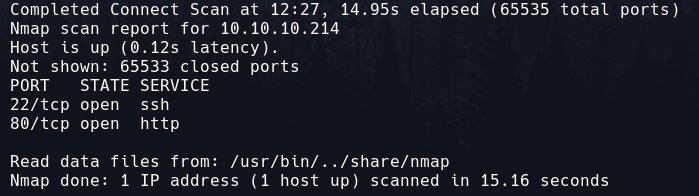
\includegraphics[width=\textwidth]{images/time/nmap.png}
	\caption{escaneo con nmap}
\end{figure}
Entonces encontramos estos dos servicios, algo que podríamos hacer para verificar la versión de los servicios es incluir el -sV.
La razón por la cual no usamos esto desde el inicio es porque al analizar todos los puertos en algunos casos hace que se demore considerablemente más, en especial cuando descubre muchos puertos.
\begin{figure}[H]
	\center
	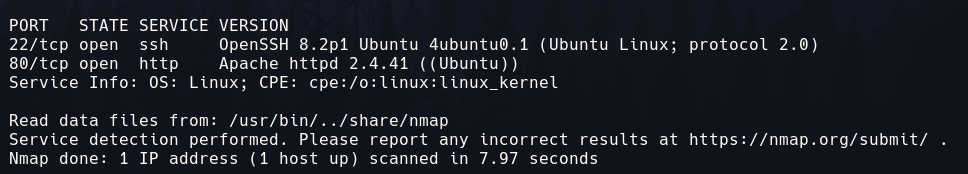
\includegraphics[width=\textwidth]{images/time/nmap_version.png}
	\caption{escaneo con version nmap}
\end{figure}
Un parámetro adicional que podríamos usar para este análisis es el :
\begin{itemize}
	\item -sV 
	\item -Pn 
	\item --script=Vuln
\end{itemize}
\clearpage
Analizamos ahora los directorios para ver si encontramos algo con gobuster, esto podría ayudarnos a encontrar alguna carpeta oculta antes de revisar el contenido, para esto usamos un parámetro importante que es el -t 200 que ayuda a que use más hilos. 
\begin{figure}[H]
	\center
	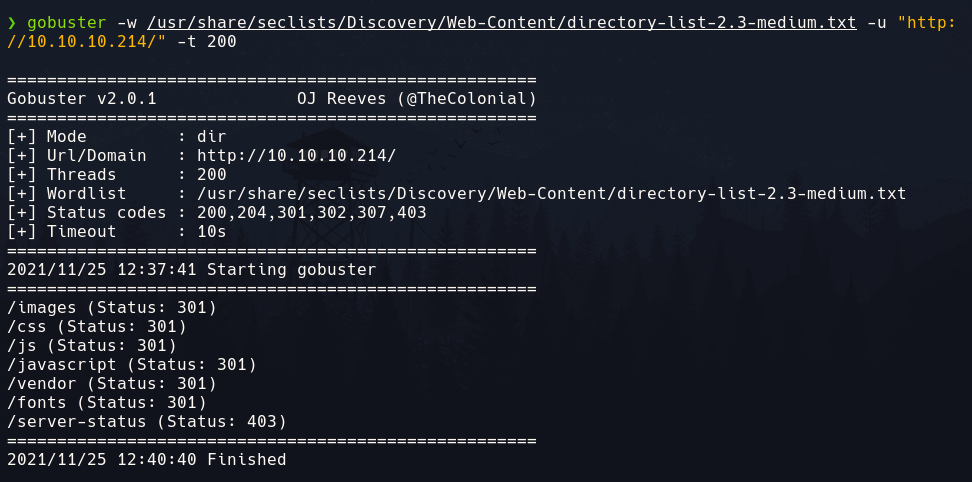
\includegraphics[width=\textwidth]{images/time/gobuster.png}
	\caption{fuzzeo con gobuster}
\end{figure}
Mientras tanto analizamos también la página web que tenemos en el puerto 80, nos encontramos con un validador de json como los que solemos encontrar en internet.
\begin{figure}[H]
	\center
	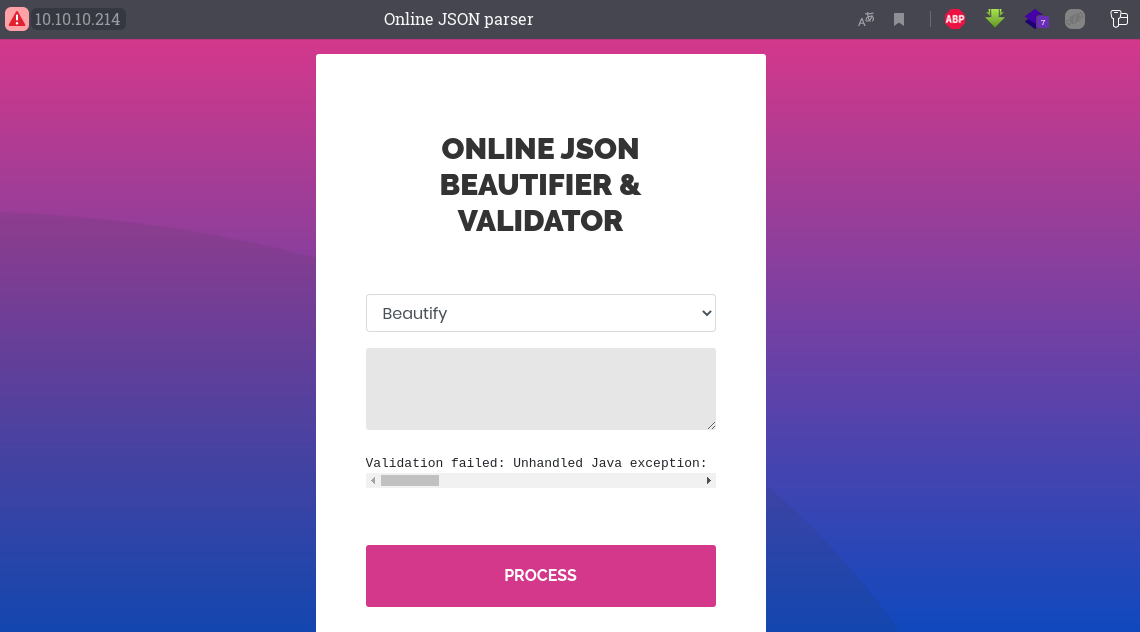
\includegraphics[width=\textwidth]{images/time/index.png}
	\caption{página de json}
\end{figure}
\clearpage
Entonces tenemos este validador, probamos metiendo un poco de código json, obtenemos este código de \href{https://json.org/example.html}{https://json.org/example.html}.
Seleccionamos dos códigos para hacer la prueba porque ambos botaban errores diferentes:
\begin{lstlisting}[language={[ANSI]C}]  
	{"title": "Sample Konfabulator Widget",
    	"name": "main_window",
    	"width": 500,
    	"height": 500}
\end{lstlisting}
Con este código te bota el siguiente error:
\begin{lstlisting}[language={[ANSI]C}] 
	Validation failed:    "title": "Sample Konfabulator Widget",
\end{lstlisting}

Luego probamos con este código de una línea a ver si había diferencia
\begin{lstlisting}[language={[ANSI]C}]  
	{"value": "New", "onclick": "CreateNewDoc()"}
\end{lstlisting}

Con este código te bota el siguiente error:
\begin{lstlisting}[language={[ANSI]C}]  
	Validation failed: Unhandled Java exception: com.fasterxml.jackson.databind.
	exc.MismatchedInputException: Unexpected token (START_OBJECT), 
	expected START_ARRAY: need JSON Array to contain As.WRAPPER_ARRAY type 
	information for class java.lang.Object
\end{lstlisting}

Entonces el segundo error nos da algo más significativo, buscando en google encontramos algunas vulnerabilidades.
\subsection{Explotación}

\subsection{Escalamiento de privilegios}


\subsection{Post Explotación}

\subsection{Hardening}

% ----------------------------Jarvis-----------------------------------
\section{Jarvis}
\subsection{Enumeración}

\subsection{Explotación}

\subsection{Escalamiento de privilegios}


\subsection{Post Explotación}

\subsection{Hardening}


\end{document}
